\phantomsection\addcontentsline{toc}{section}{\numberline {}CHƯƠNG 3. THIẾT KẾ CHUYỂN ĐỔI PDM SANG PCM NHIỀU GIAI ĐOẠN VÀ KIỂM THỬ BẰNG PHẦN MỀM}
\section*{CHƯƠNG 3. THIẾT KẾ CHUYỂN ĐỔI PDM SANG PCM NHIỀU GIAI ĐOẠN VÀ KIỂM THỬ BẰNG PHẦN MỀM} \label{chuong3}
\setcounter{section}{3}
\setcounter{subsection}{0}
\setcounter{figure}{0}
\setcounter{table}{0}
Ở \hyperref[chuong2]{chương 2}, chúng ta đã trình bày thảo luận về bộ chuyển đổi Sigma-Delta, phổ của tín hiệu PDM từ micro, các bộ lọc khác nhau và cách tìm ra các hệ số phù hợp cho các bộ lọc đó. Chương này mô tả các yêu cầu thiết kế, cách kết hợp tất cả lại với nhau, tạo ra bộ chuyển đổi PDM sang PCM nhiều giai đoạn và kiểm thử thiết kế bằng ngôn ngữ \textit{Python}.
\subsection{Yêu cầu thiết kế} \label{spec_muc}
Qua những gì đã giới thiệu về MEMS ở mục \ref{micro}, chúng ta đưa ra những yêu cầu thiết kế sau:
\begin{itemize}
    \item Tốc độ lấy mẫu ở đầu ra (PCM) là 48 kHz.\\
    Tốc độ lấy mẫu 48 kHz là tốc độ phổ biến dùng cho các âm thanh chất lượng cao
    \item Tốc độ lấy mẫu PDM là 2.304 MHz.\\
    Micrô hỗ trợ tốc độ xung nhịp PDM trong khoảng từ 1 đến 3,25 MHz. Có các bộ lọc rất hiệu quả cho phép Decimation 2x, vì vậy nên chọn một tỷ lệ decimation là một số chia hết cho lũy thừa của 2. Tỷ lệ 48x được cho là phù hợp nhất.
    \item Băng thông từ 0 đến 6kHz.\\
    Với việc âm thanh thu được chỉ ổn định trong tần số 100Hz đến 5kHz, điểm chuyển tiếp ở vị trí 6kHz là một điểm phù hợp.
    \item Dải dừng bắt đầu ở 10kHz: vì ở trên tần số 10kHz, micro không có hành vi gì.
    \item SNR của tín hiệu đầu ra là 87 dB: Giảm so với Dynamic Range 1 dB
    \item Độ gợn sóng là 0.1 dB: yêu cầu cần thiết đối với âm thanh chất lượng cao.
\end{itemize}
Độ suy hao của dải dừng sẽ được tính theo công thức \ref{stopband} \cite{pdm2pcm}.
\begin{equation} \label{stopband}
    A_{stop band} = -3dB - 10log_{10}{(10^{-\displaystyle\frac{SNR_{after}}{10}}-10^{-\displaystyle\frac{SNR_{before}}{10}})}
\end{equation}
Từ đó, chúng ta tóm tắt các yêu cầu thiết kế như bảng \ref{spec}.
\begin{table}[H]
    \centering
    \caption[Các yêu cầu thiết kế của hệ thống]{\bfseries\fontsize{12pt}{0pt}\selectfont Các yêu cầu thiết kế của hệ thống}
    \begin{tabular}{|l|c|c|}
        \hline
        \multicolumn{1}{|c|}{\textbf{Yêu cầu}}                                  & \textbf{Thông tin} & \textbf{Đơn vị} \\ \hline
        \begin{tabular}[c]{@{}l@{}}Tốc độ lấy mẫu đầu vào \\ (PDM)\end{tabular} & 2304               & MHz             \\ \hline
        \begin{tabular}[c]{@{}l@{}}Tốc độ lấy mẫu đầu ra\\ (PCM)\end{tabular}   & 48                 & kHz             \\ \hline
        Hệ số decimation                                                        & 48                 & lần             \\ \hline
        Dải thông                                                               & 0 - 6                & kHz             \\ \hline
        Dải dừng                                                                & 10                  & kHz             \\ \hline
        Độ gợn sóng dải thông         & 0.1                & dB              \\ \hline
        Độ suy hao của dài dừng                                                 & 89                 & dB              \\ \hline
    \end{tabular}
    \label{spec}
\end{table}

\subsection{Thiết kế bộ chuyển đổi PDM sang PCM}
Khi chúng ta quan sát phổ của tín hiệu PDM, các nhiễu lượng tử sẽ được dồn sang ở tần số cao, còn phần cần lấy thông tin sẽ ở trong một khoảng tần số thấp nhất định. Cho nên, bộ chuyển đổi sẽ chỉ cần 2 bước cơ bản (hình \ref{pdm2pcm_top}):
\begin{enumerate}
    \item Gửi tín hiệu PDM thông qua một bộ lọc thông thấp. Nó sẽ loại bỏ tất cả các nhiễu ở tần số cao.
    \item Sử dụng kỹ thuật Decimation (hạ tần) để các mẫu được lấy mẫu với tỷ lệ thấp hơn. Việc sử dụng bộ lọc thông thấp từ bước 1 cũng sẽ giúp tránh được hiện tượng chồng phổ.
\end{enumerate}

\begin{figure}[H]
    \centering
    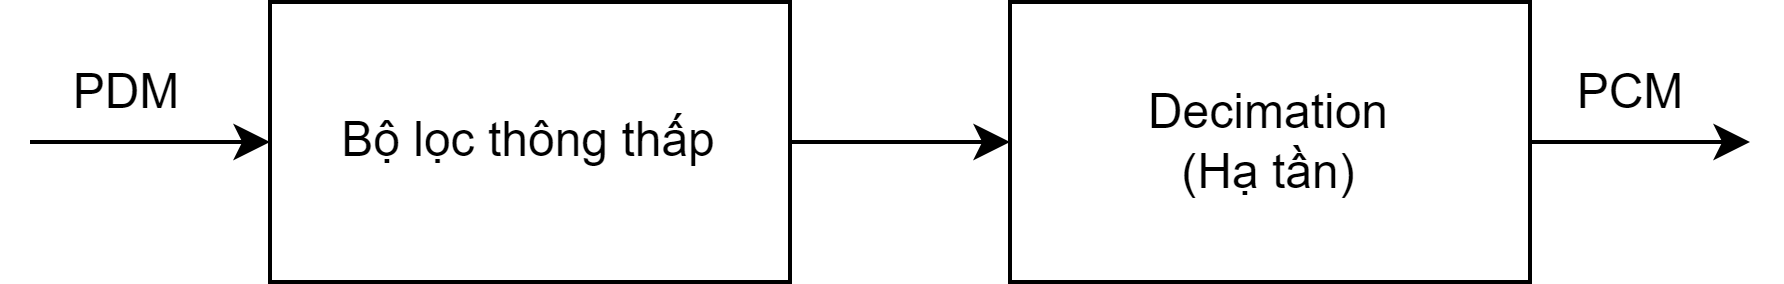
\includegraphics[width=12cm]{Images/Chuong3/pdm2pcm_top.png}
    \caption[Sơ đồ tổng quát của bộ chuyển đổi]{\bfseries \fontsize{12pt}{0pt}\selectfont Sơ đồ tổng quát của bộ chuyển đổi}
    \label{pdm2pcm_top}
\end{figure}
Ở trong đề tài này, chúng ta sẽ thiết kế bộ lọc "Equiripple" bằng thuật toán \textbf{Parks-McClellan} \cite{rao2018digital}. Trong thư viện \textit{Numpy} đã có sẵn chức năng \textit{remez} để thiết kế các bộ lọc theo thông số được đặt ra, việc triển khai sẻ sử dụng ngôn ngữ \textit{Python}.
\subsubsection{Ý tưởng thiết kế đơn giản} \label{dongian}
Không thực sự cần một kiến trúc bộ lọc phức tạp để chuyển đổi PDM sang PCM, chúng ta chỉ cần 1 bộ lọc thông thấp duy nhất là đã có thể đáp ứng được các thông số ở trên.

Bộ lọc thông thấp sẽ có các thông số như sau: 
\begin{itemize}
    \item Dải thông: 0 - 6 kHz
    \item Dải dừng: 10 kHz - 2304kHz
    \item Độ suy hao dải dừng: 89dB
    \item Độ gợn sóng của dải thông: 0.1dB
\end{itemize}

Sau tiến hành chạy thuật toán \textit{remez}, chúng ta có bộ lọc có 2116 taps,  biểu đồ đáp ứng tần số và đáp ứng xung mô tả lần lượt ở hình \ref{filter_the_damn_thing} và \ref{filter_the_damn_thing_impulse}.
\begin{figure}[H]
    \centering
    \includesvg[width=14cm]{Images/Chuong3/filter_the_damn_thing.svg}
    \caption[Đáp ứng tần số của bộ lọc đơn giản]{\bfseries \fontsize{12pt}{0pt}\selectfont Đáp ứng tần số của bộ lọc đơn giản}
    \label{filter_the_damn_thing}
\end{figure}
\begin{figure}[H]
    \centering
    \includesvg[width=14cm]{Images/Chuong3/filter_the_damn_thing_impulse.svg}
    \caption[Đáp ứng xung của bộ lọc đơn giản]{\bfseries \fontsize{12pt}{0pt}\selectfont Đáp ứng xung của bộ lọc đơn giản}
    \label{filter_the_damn_thing_impulse}
\end{figure}

Bộ trên có độ suy hao dải dừng là 89.035 dB, độ gợn sóng 0.01415 dB hoàn toàn thỏa mãn với yêu cầu thiết kế. Nhưng có một vấn đề, đó là số taps lớn dẫn đến phép nhân trong 1 giây khá lớn ($48000 \times 2216 = 106M \text{ phép}/s$). Trong thiết kế phần cứng, đồng nghĩa chúng ta phải dùng đến 2216 bộ nhân, điều đó gây nên hao phí tài nguyên nghiêm trọng.

\textbf{Kết luận}: việc sửa dụng một bộ lọc thông thấp duy nhất không được cho là khả thi. Phần sau sẽ trình bày kiểu thiết kế sử dụng nhiều bộ lọc tối ưu và xử lý ở nhiều miền tần số.

\subsubsection{Thiết kế bộ chuyển đổi nhiều giai đoạn sử dụng hạ tần (Decimation)}
Có rất nhiều kiến trúc đường ống để khử tín hiệu mẫu ở tốc độ cao xuống thấp \cite{pipelie1} - \cite{pipelie2}, về cơ bản sẽ được rút gọn thành các khối như hình \ref{pipeline_top}:
\begin{itemize}
    \item Một bộ lọc CIC phía trước
    \item Một hoặc nhiều bộc lọc Half Band ở giữa
    \item Một bộ lọc FIR ở phía sau
\end{itemize}

\begin{figure}[H]
    \centering
    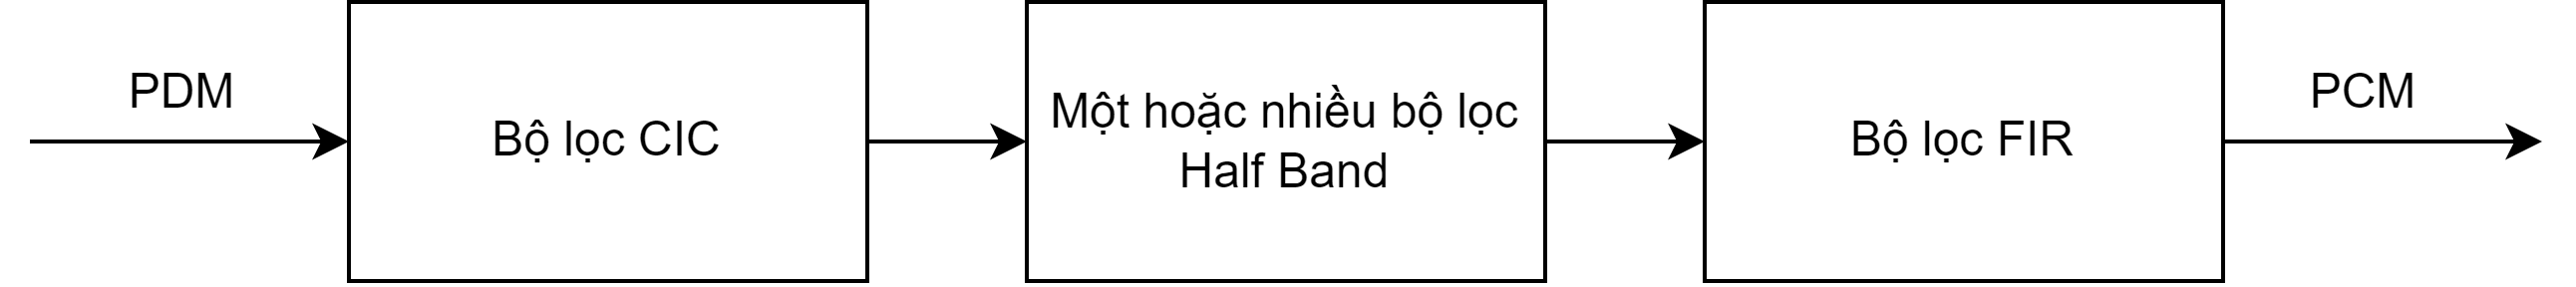
\includegraphics[width=15cm]{Images/Chuong3/pipeline_top.png}
    \caption[Sơ đồ khối của thiết kế dạng nhiều giai đoạn]{\bfseries \fontsize{12pt}{0pt}\selectfont Sơ đồ khối của thiết kế dạng nhiều giai đoạn}
    \label{pipeline_top}
\end{figure}
Lý do cho sự sắp xếp này là để phù hợp ràng buộc thiết kế như tốc độ xung nhịp và đặc biệt là mức sử dụng tài nguyên.
\begin{itemize}
    \item Bộ lọc CIC chỉ yêu cầu bộ cộng và bộ trễ chứ không yêu cầu bộ nhân. Điều này là cho thiết kế giảm đi một diện tích đáng kể.
    \item Việc không sử dụng bộ nhân cũng làm cho bộ lọc CIC dễ dàng chạy được ở tần số cao
    \item Bộ lọc hand Band chỉ yêu cầu khoảng 50\% phép nhân so với bộ lọc FIR tương đương.
    \item Việc sử dụng 2 bộ lọc CIC và Half Band vẫn chưa đủ điều kiện để lọc triệt để tín hiệu cần thu, dẫn đến việc phải sử dụng bộ FIR sau cùng. Nhưng bộ lọc này chạy ở tần số thấp và tài nguyên là không đáng kể.
\end{itemize}
\paragraph{Cấu hình bộ lọc CIC}
Vì bộ lọc CIC không sử dụng bất kỳ bộ nhân nào, các thông số của bộ lọc chỉ phụ thuộc vào 2 tham số là số tầng và kích thước cửa số. Tuy nhiên, các bộ lọc CIC có độ gợn của dải thông trở nên ngày càng tồi tệ hơn với tần số tăng và số lượng các tầng tăng.

Do yêu cầu thiết kế có hệ số decimation là 48, do đó có 9 tỷ lệ có thể được chọn cho CIC: 2 3 4 6 8 12 16 24 48.

Hình \ref{cic_ratios_overview} mô tả đáp ứng tần số của bộ lọc CIC với tất cả các tỷ lệ decimation nói trên và 5 tầng. Gạch nối màu đỏ biểu thị ranh giới 6 kHz cần thu tín hiệu, chúng ta tiếp tục phân tích bằng cách phóng to (hình \ref{cic_ratios_zoom}). Dễ dành nhận ra ở dải tần 0 - 6 kHz và độ gợn sóng 0.1 dB, tỷ lệ Decimation từ 16 trở đi vi phạm yêu cầu thiết kế đặt ra. Điều đó có thể khắc phục bằng cách tăng số tầng của bộ lọc nhưng sẽ có một rắc rối đó là sẽ làm giảm độ suy hao của dải dừng.

\begin{figure}[H]
    \centering
    \includesvg[width=15cm]{Images/Chuong3/cic_ratios_overview.svg}
    \caption[Đáp ứng tần số của bộ lọc CIC 5 tầng với tất cả hệ số Decimation]{\bfseries \fontsize{12pt}{0pt}\selectfont Đáp ứng tần số của bộ lọc CIC 5 tầng với tất cả hệ số Decimation}
    \label{cic_ratios_overview}
\end{figure}

\begin{figure}[H]
    \centering
    \includesvg[width=15cm]{Images/Chuong3/cic_ratios_zoom.svg}
    \caption[Đáp ứng tần số của bộ lọc CIC 5 tầng với tất cả hệ số Decimation (phóng to)]{\bfseries \fontsize{12pt}{0pt}\selectfont Đáp ứng tần số của bộ lọc CIC 5 tầng với tất cả hệ số Decimation (phóng to)}
    \label{cic_ratios_zoom}
\end{figure}

Để đơn giản, chúng ta sẽ phải giới hạn tỷ lệ decimation số lượng các tầng sao cho độ gợn dải thông không vượt quá một giá trị tối đa nhất định. Ở đây sẽ chọn độ gợn tối đa là 0.05 dB.

Để tìm ra thông số CIC thỏa mãn cả yêu cầu về dải thông và dải dừng, chúng ta sẽ tập trung vào bảng \ref{abc}. Nên chọn số tầng thấp nhất có thể để giảm được số lượng độ rộng của thanh ghi và các bộ cộng. Từ đó có thể đáp ứng được vấn đề về tài nguyên của hệ thống số.

 \noindent Từ bảng \ref{abc}, các phương án sau được đưa ra:
\begin{itemize}
    \item Tỷ lệ Decimation 6x và số tầng 3: phương án này yêu cầu thêm 3 bộ lọc Half Band và 1 bộ lọc FIR cuối để đáp ứng được các thông số cuối cùng.
    \item Tỷ lệ Decimation 8x và số tầng 4: phương án này yêu cần cần thêm tỷ lệ Decimation phía sau là 6x, đồng nghĩa với dùng 1 bộ lọc Half Band và 1 bộ lọc FIR cuối kèm theo 1 bộ decimation 3x.
    \item Tỷ lệ Decimation 12x và số tầng 4: mặc dùng phương án này chưa đáp ứng được độ gợn sóng của dải thông (0.056 db, vượt 0.006 dB so với yêu cầu), nhưng chênh lệch này rất nhỏ. Với phương án này yêu cầu thêm 2 bộ lọc Half Band và 1 bộ lọc FIR. \label{choose}
\end{itemize}
\vspace{2.5cm}
\begin{table}[H]
    \centering
    \caption[Độ gợn sóng và độ suy hao của dải dừng của bộ lọc CIC ở nhiều cấu hình khác nhau (dB)]{\bfseries\fontsize{12pt}{0pt}\selectfont Độ gợn sóng và độ suy hao của dải dừng của bộ lọc CIC ở nhiều cấu hình khác nhau (dB)}
\begin{tabular}{|c|l|l|l|l|l|l|}
\hline
\backslashbox{\textbf{Tỷ lệ}}{\textbf{Tầng}} &
  \multicolumn{1}{c|}{\textbf{1}} &
  \multicolumn{1}{c|}{\textbf{2}} &
  \multicolumn{1}{c|}{\textbf{3}} &
  \multicolumn{1}{c|}{\textbf{4}} &
  \multicolumn{1}{c|}{\textbf{5}} &
  \multicolumn{1}{c|}{\textbf{6}} \\ \hline
\textbf{2} &
  \begin{tabular}[c]{@{}l@{}}-0,0003\\ -37,3\end{tabular} &
  \begin{tabular}[c]{@{}l@{}}-0,0006\\ -74,6\end{tabular} &
  \begin{tabular}[c]{@{}l@{}}-0,0009\\ -112,0\end{tabular} &
  \begin{tabular}[c]{@{}l@{}}-0,0012\\ -149,3\end{tabular} &
  \begin{tabular}[c]{@{}l@{}}-0,0015\\ -186,6\end{tabular} &
  \begin{tabular}[c]{@{}l@{}}-0,0018\\ -223,9\end{tabular} \\ \hline
\textbf{3} &
  \begin{tabular}[c]{@{}l@{}}-0,0008\\ -36,0\end{tabular} &
  \begin{tabular}[c]{@{}l@{}}-0,0016\\ -72,0\end{tabular} &
  \begin{tabular}[c]{@{}l@{}}-0,0024\\ -108,0\end{tabular} &
  \begin{tabular}[c]{@{}l@{}}-0,0032\\ -144,0\end{tabular} &
  \begin{tabular}[c]{@{}l@{}}-0,0039\\ -180,0\end{tabular} &
  \begin{tabular}[c]{@{}l@{}}-0,0047\\ -216,0\end{tabular} \\ \hline
\textbf{4} &
  \begin{tabular}[c]{@{}l@{}}-0,0015\\ -34,2\end{tabular} &
  \begin{tabular}[c]{@{}l@{}}-0,0030\\ -68,4\end{tabular} &
  \begin{tabular}[c]{@{}l@{}}-0,0044\\ -102,6\end{tabular} &
  \begin{tabular}[c]{@{}l@{}}-0,0059\\ -136,8\end{tabular} &
  \begin{tabular}[c]{@{}l@{}}-0,0074\\ -171,0\end{tabular} &
  \begin{tabular}[c]{@{}l@{}}-0,0089\\ -205,2\end{tabular} \\ \hline
\textbf{6} &
  \begin{tabular}[c]{@{}l@{}}-0,0034\\ -31,1\end{tabular} &
  \begin{tabular}[c]{@{}l@{}}-0,0069\\ -62,2\end{tabular} &
  \begin{tabular}[c]{@{}l@{}}-0,0103\\ -93,3\end{tabular} &
  \begin{tabular}[c]{@{}l@{}}-0,0138\\ -124,4\end{tabular} &
  \begin{tabular}[c]{@{}l@{}}-0,0172\\ -155,5\end{tabular} &
  \begin{tabular}[c]{@{}l@{}}-0,0207\\ -186,6\end{tabular} \\ \hline
\textbf{8} &
  \begin{tabular}[c]{@{}l@{}}-0,0062\\ -28,7\end{tabular} &
  \begin{tabular}[c]{@{}l@{}}-0,0124\\ -57,4\end{tabular} &
  \begin{tabular}[c]{@{}l@{}}-0,0186\\ -86,1\end{tabular} &
  \begin{tabular}[c]{@{}l@{}}-0,0248\\ -114,8\end{tabular} &
  \begin{tabular}[c]{@{}l@{}}-0,0310\\ -143,5\end{tabular} &
  \begin{tabular}[c]{@{}l@{}}-0,0372\\ -172,2\end{tabular} \\ \hline
\textbf{12} &
  \begin{tabular}[c]{@{}l@{}}-0,0141\\ -25,2\end{tabular} &
  \begin{tabular}[c]{@{}l@{}}-0,0282\\ -50,3\end{tabular} &
  \begin{tabular}[c]{@{}l@{}}-0,0423\\ -75,5\end{tabular} &
  \begin{tabular}[c]{@{}l@{}}-0,0564\\ -100,6\end{tabular} &
  \begin{tabular}[c]{@{}l@{}}-0,0705\\ -125,8\end{tabular} &
  \begin{tabular}[c]{@{}l@{}}-0,0846\\ -150,9\end{tabular} \\ \hline
\textbf{16} &
  \begin{tabular}[c]{@{}l@{}}-0,0251\\ -22,6\end{tabular} &
  \begin{tabular}[c]{@{}l@{}}-0,0502\\ -45,2\end{tabular} &
  \begin{tabular}[c]{@{}l@{}}-0,0753\\ -67,7\end{tabular} &
  \begin{tabular}[c]{@{}l@{}}-0.1004\\ -90.3\end{tabular} &
  \begin{tabular}[c]{@{}l@{}}-0,1256\\ -112,9\end{tabular} &
  \begin{tabular}[c]{@{}l@{}}-0,1507\\ -135,5\end{tabular} \\ \hline
\textbf{24} &
  \begin{tabular}[c]{@{}l@{}}-0,0568\\ -18,8\end{tabular} &
  \begin{tabular}[c]{@{}l@{}}-0,1135\\ -37,7\end{tabular} &
  \begin{tabular}[c]{@{}l@{}}-0,1703\\ -56,5\end{tabular} &
  \begin{tabular}[c]{@{}l@{}}-0,2271\\ -75,3\end{tabular} &
  \begin{tabular}[c]{@{}l@{}}-0,2839\\ -94,2\end{tabular} &
  \begin{tabular}[c]{@{}l@{}}-0,3406\\ -113,0\end{tabular} \\ \hline
\textbf{48} &
  \begin{tabular}[c]{@{}l@{}}-0,2190\\ -12,2\end{tabular} &
  \begin{tabular}[c]{@{}l@{}}-0,4381\\ -24,4\end{tabular} &
  \begin{tabular}[c]{@{}l@{}}-0,6571\\ -36,6\end{tabular} &
  \begin{tabular}[c]{@{}l@{}}-0,8761\\ -48,8\end{tabular} &
  \begin{tabular}[c]{@{}l@{}}-1,0952\\ -61,0\end{tabular} &
  \begin{tabular}[c]{@{}l@{}}-1.3142\\ -73.2\end{tabular} \\ \hline
\end{tabular}
\label{abc}
\end{table}

\begin{table}[H]
    \centering
    \caption[Bảng tính toán tổng các phép nhân của từng phương án]{\bfseries\fontsize{12pt}{0pt}\selectfont Bảng tính toán tổng các phép nhân của từng phương án}
\begin{tabular}{|c|l|l|l|l|l|}
\hline
\textbf{Phương án} &
  \multicolumn{1}{c|}{\textbf{\begin{tabular}[c]{@{}c@{}}HB1\\ (phép/s)\end{tabular}}} &
  \multicolumn{1}{c|}{\textbf{\begin{tabular}[c]{@{}c@{}}HB2\\ (phép/s)\end{tabular}}} &
  \multicolumn{1}{c|}{\textbf{\begin{tabular}[c]{@{}c@{}}HB3\\ (phép/s)\end{tabular}}} &
  \multicolumn{1}{c|}{\textbf{\begin{tabular}[c]{@{}c@{}}FIR\\ (phép/s)\end{tabular}}} &
  \multicolumn{1}{c|}{\textbf{\begin{tabular}[c]{@{}c@{}}Tổng\\ (phép/s)\end{tabular}}} \\ \hline
\textbf{Phương án 1} &
  \begin{tabular}[c]{@{}l@{}}4 x 192 k\\ =768 k\end{tabular} &
  \begin{tabular}[c]{@{}l@{}}6 x 96 k\\ = 576 k\end{tabular} &
  \begin{tabular}[c]{@{}l@{}}10 x 48 k\\ = 480 k\end{tabular} &
  \begin{tabular}[c]{@{}l@{}}47 x 48 k\\ = 2256 k\end{tabular} &
  4080 k \\ \hline
\textbf{Phương án 2} &
  \begin{tabular}[c]{@{}l@{}}6 x 144 k\\ = 864 k\end{tabular} &
   &
   &
  \begin{tabular}[c]{@{}l@{}}141 x 48 k\\ = 6768 k\end{tabular} &
  4320 k \\ \hline
\textbf{Phương án 3} &
  \begin{tabular}[c]{@{}l@{}}6 x 96 k\\ = 576 k\end{tabular} &
  \begin{tabular}[c]{@{}l@{}}10 * 48 k \\ = 480 k\end{tabular} &
   &
  \begin{tabular}[c]{@{}l@{}}51 x 48 k\\ = 2448 k\end{tabular} &
  3504 k \\ \hline
\end{tabular}
\label{phepnhan}
\end{table}
Khi các thuộc tính của bộ lọc CIC đã được quyết định, thiết kế bộ lọc Half Band và FIR sẽ được chạy thuật toán Parks-McClellan/Remez để đưa ra các hệ số bộ lọc chính xác. Từ đó, chúng ta có thể đưa ra số phép nhân xảy ra trong 1 giây, mô tả như bảng \ref{phepnhan}. Dễ dàng nhận ra phương án 3 là phương án tối ưu nhất.

Giờ thì chúng ta có thể thấy rõ sự khác biệt giữa 2 kiến trúc đơn giản (mục \ref{dongian}) và sử dụng nhiều bộ lọc trên nhiều miền tần số khác nhau. Với 3504k phép nhân trên 1 giây so với 106M phép nhân trong 1 giây, nó được cải thiện hơn 30 lần.
\subsubsection{Thiết kế bộ lọc Half Band và FIR}
Với phương án \hyperref[choose]{đã được chọn ở trên}, chúng ta có sơ đồ khối tổng quát của thiết kế như hình \ref{pipeline_new}.
\begin{figure}[H]
    \centering
    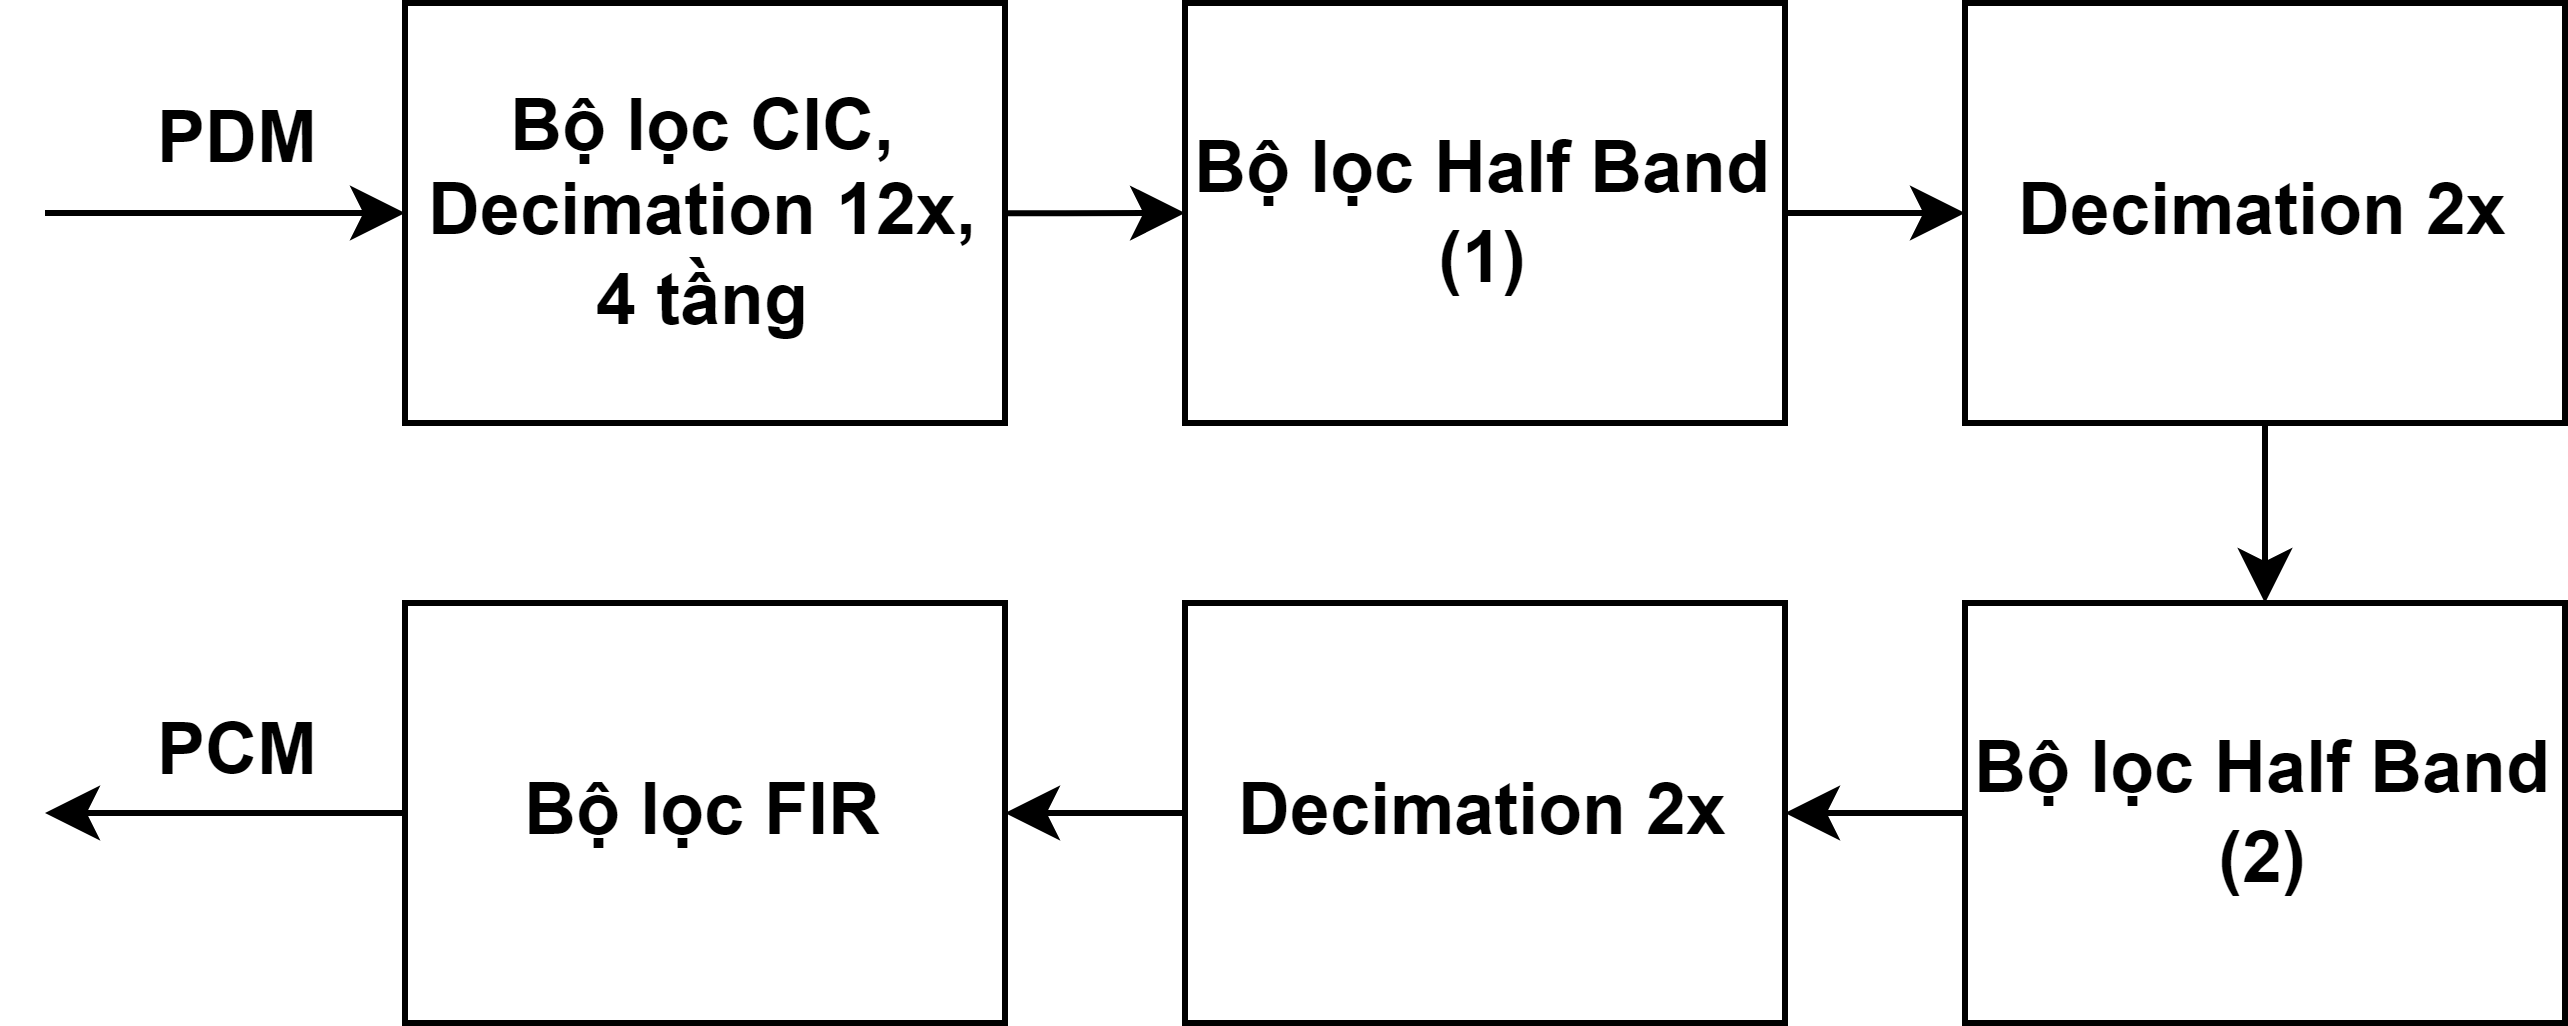
\includegraphics[width=11cm]{Images/Chuong3/pipeline_new_top.png}
    \caption[Sơ đồ khối tổng quát của bộ chuyển đổi nhiều giai đoạn]{\bfseries \fontsize{12pt}{0pt}\selectfont Sơ đồ khối tổng quát của bộ chuyển đổi nhiều giai đoạn}
    \label{pipeline_new}
\end{figure}
 \noindent Các bộ lọc sẽ phải đạt các thông số thiết kế tối thiểu như sau:
\begin{enumerate}
    \item Bộ lọc CIC: \\
    Hệ số Decimation: 12\\
    Số tầng: 4\\
    Độ gợn sóng của dải thông: $A_{CIC} =$ 0.0564 dB\\
    Tần số lấy mẫu: 2304 kHz
    \item Bộ lọc Half Band (1):\\
    Tần số lấy mẫu: 192 kHz\\
    Dải thông: 0 - 10 kHz\\
    Điểm dừng: 86 kHz\\
    Độ gợn sóng của dải thông: $A_{HB1} = 0.1 - A_{CIC}$\\
    Độ suy hao của dải dừng: 89 dB
    \item Bộ lọc Half Band (2):\\
    Tần số lấy mẫu: 96 kHz\\
    Dải thông: 0 - 10 kHz\\
    Điểm dừng: 38 kHz\\
    Độ gợn sóng của dải thông: $A_{HB2} = 0.1 - A_{CIC} - A_{HB1}$\\
    Độ suy hao của dải dừng: 89 dB
    \item Bộ lọc FIR:\\
    Tần số lấy mẫu: 48 kHz\\
    Dải thông: 0 - 6 kHz\\
    Điểm dừng: 10 kHz\\
    Độ gợn sóng của dải thông: $A_{HB2} = 0.1 - A_{CIC} - A_{HB1} - A_{HB2}$\\
    Độ suy hao của dải dừng: 89 dB
\end{enumerate}

 \noindent Phổ của từng giai đoạn mô tả như hình 
 \ref{t1}, \ref{t2}, \ref{t3}, \ref{t4}.
 \vspace{2.3cm}
 \begin{figure}[H]
    \centering
    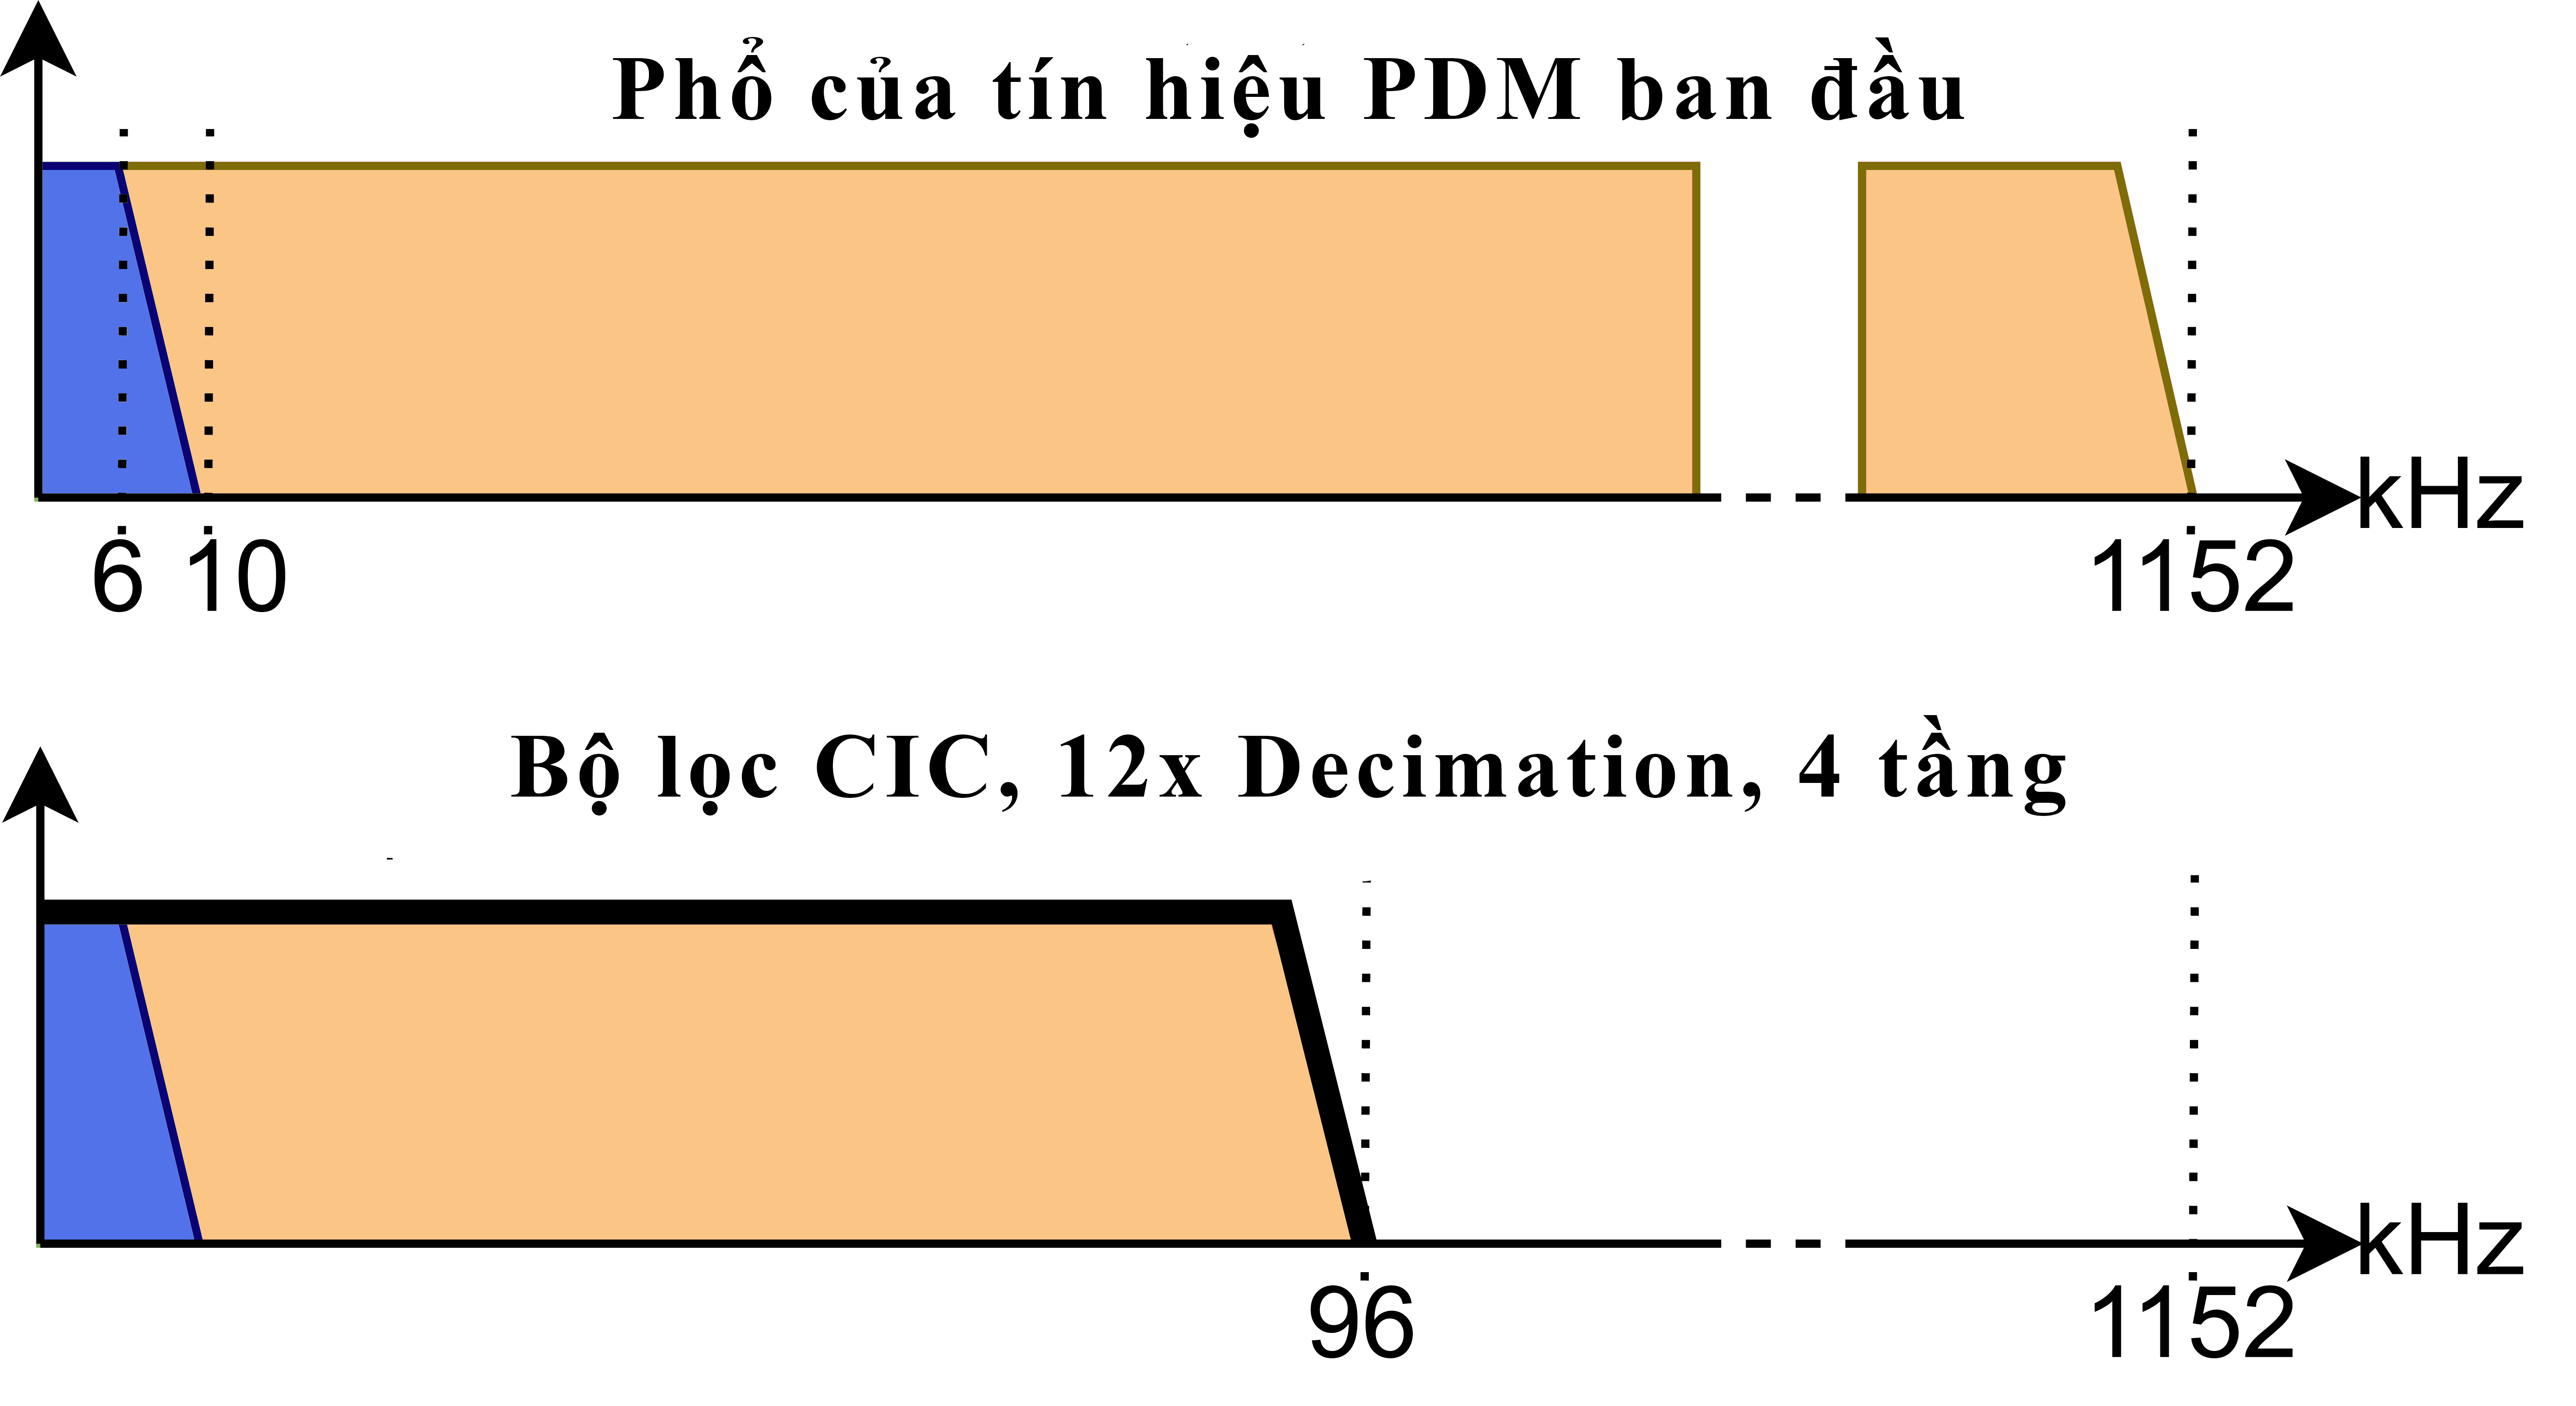
\includegraphics[width=11cm]{Images/Chuong3/1.png}
    \caption[Phổ của tín hiệu sau khi qua bộ lọc CIC]{\bfseries \fontsize{12pt}{0pt}\selectfont Phổ của tín hiệu sau khi qua bộ lọc CIC}
    \label{t1}
\end{figure}
\begin{figure}[H]
    \centering
    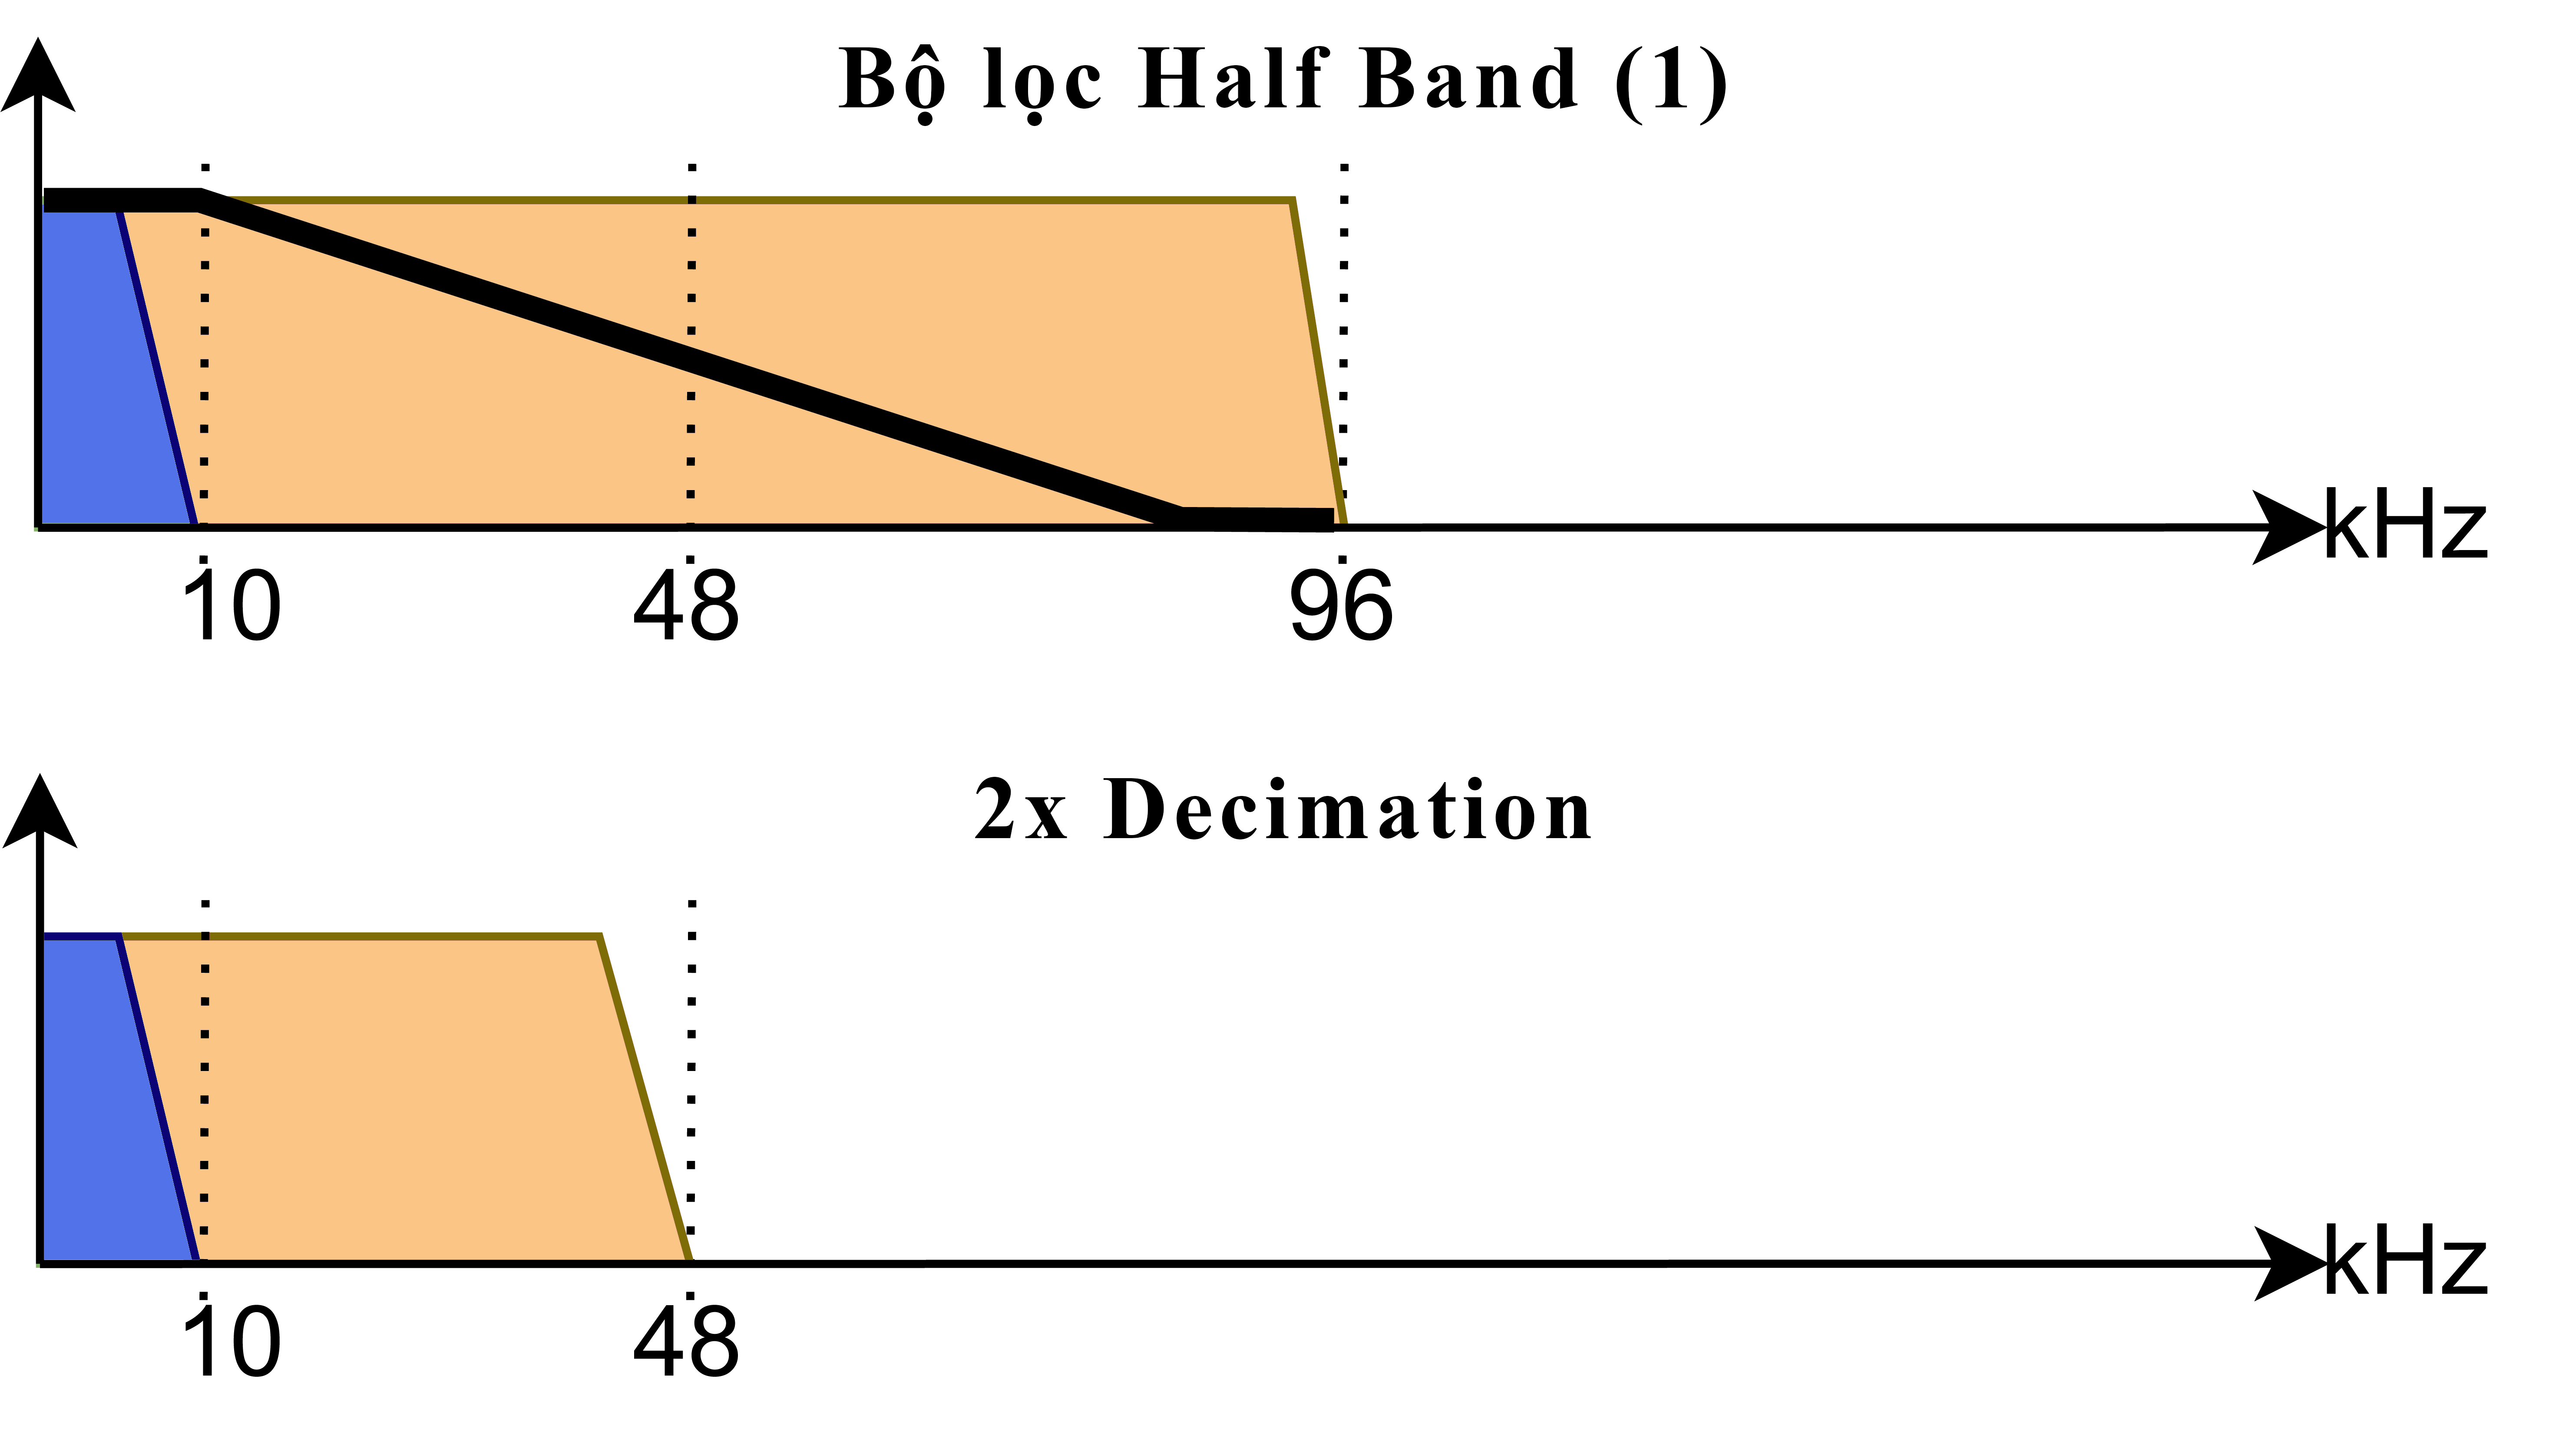
\includegraphics[width=11cm]{Images/Chuong3/2.png}
    \caption[Phổ của tín hiệu sau khi qua bộ lọc Half Band (1) và bộ Decimation 2x]{\bfseries \fontsize{12pt}{0pt}\selectfont Phổ của tín hiệu sau khi qua bộ lọc Half Band (1) và bộ Decimation 2x}
    \label{t2}
\end{figure}
\begin{figure}[H]
    \centering
    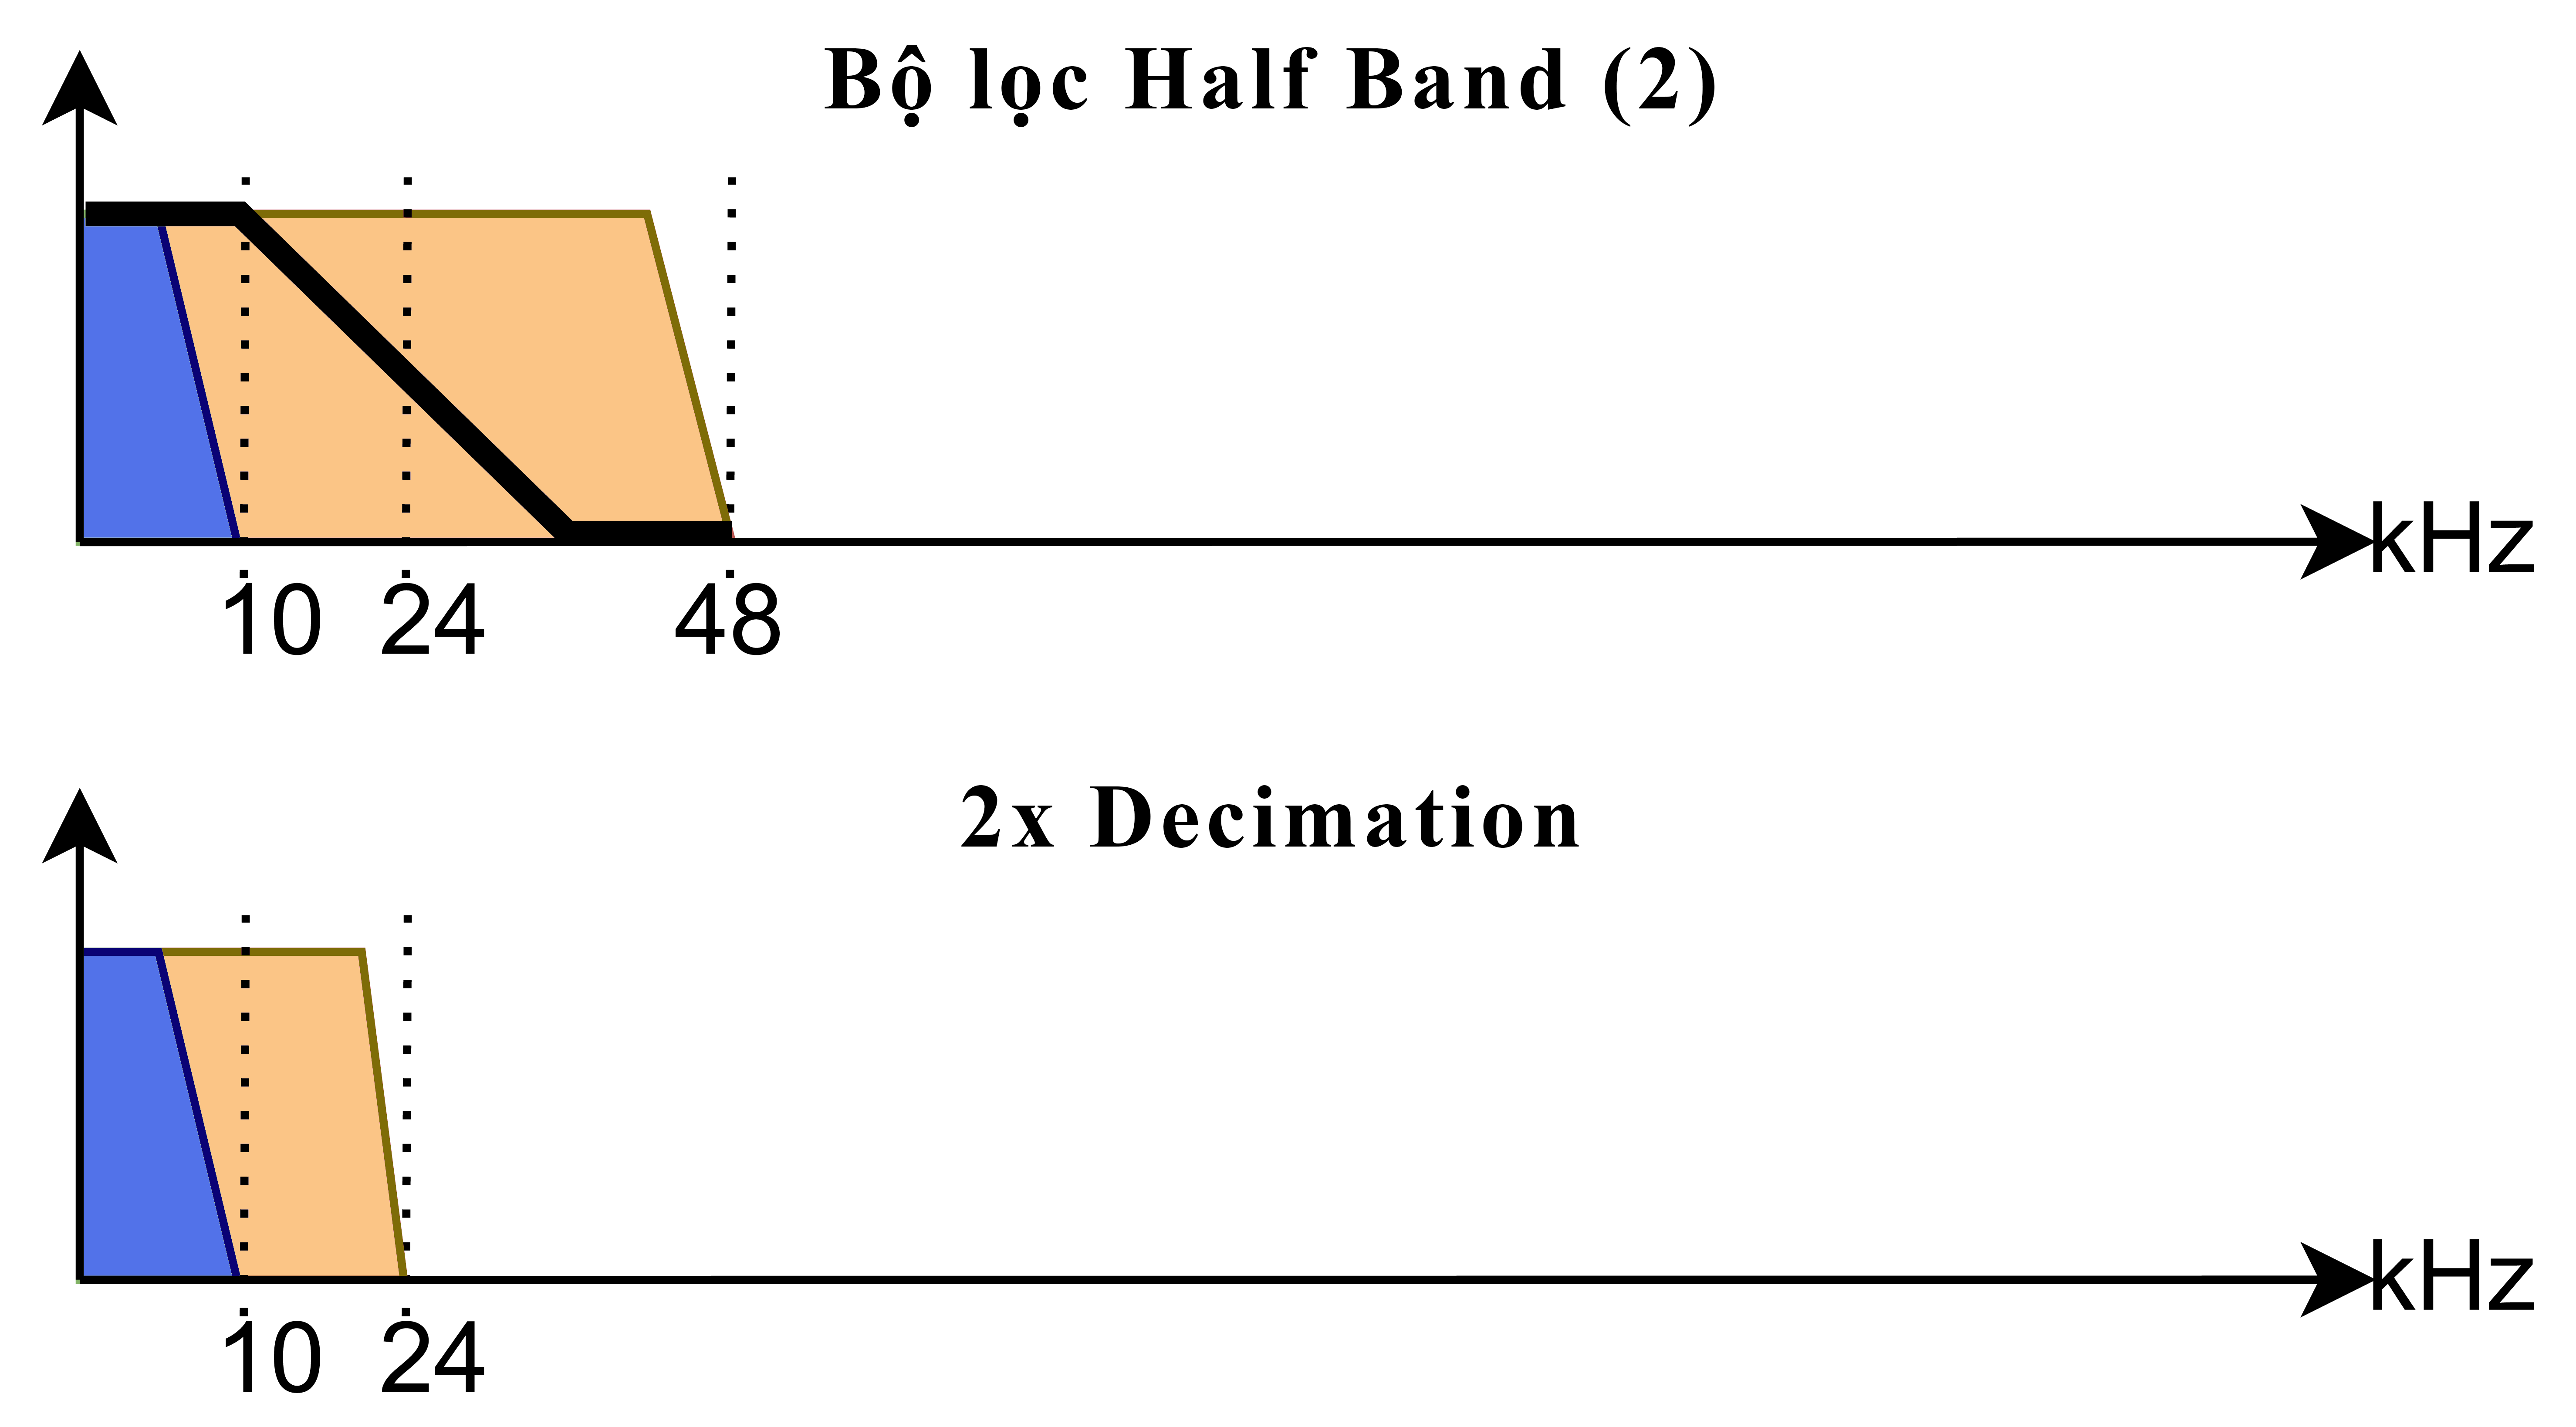
\includegraphics[width=11cm]{Images/Chuong3/3.png}
    \caption[Phổ của tín hiệu sau khi qua bộ lọc Half Band (2) và bộ Decimation 2x]{\bfseries \fontsize{12pt}{0pt}\selectfont Phổ của tín hiệu sau khi qua bộ lọc Half Band (2) và bộ Decimation 2x}
    \label{t3}
\end{figure}
\begin{figure}[H]
    \centering
    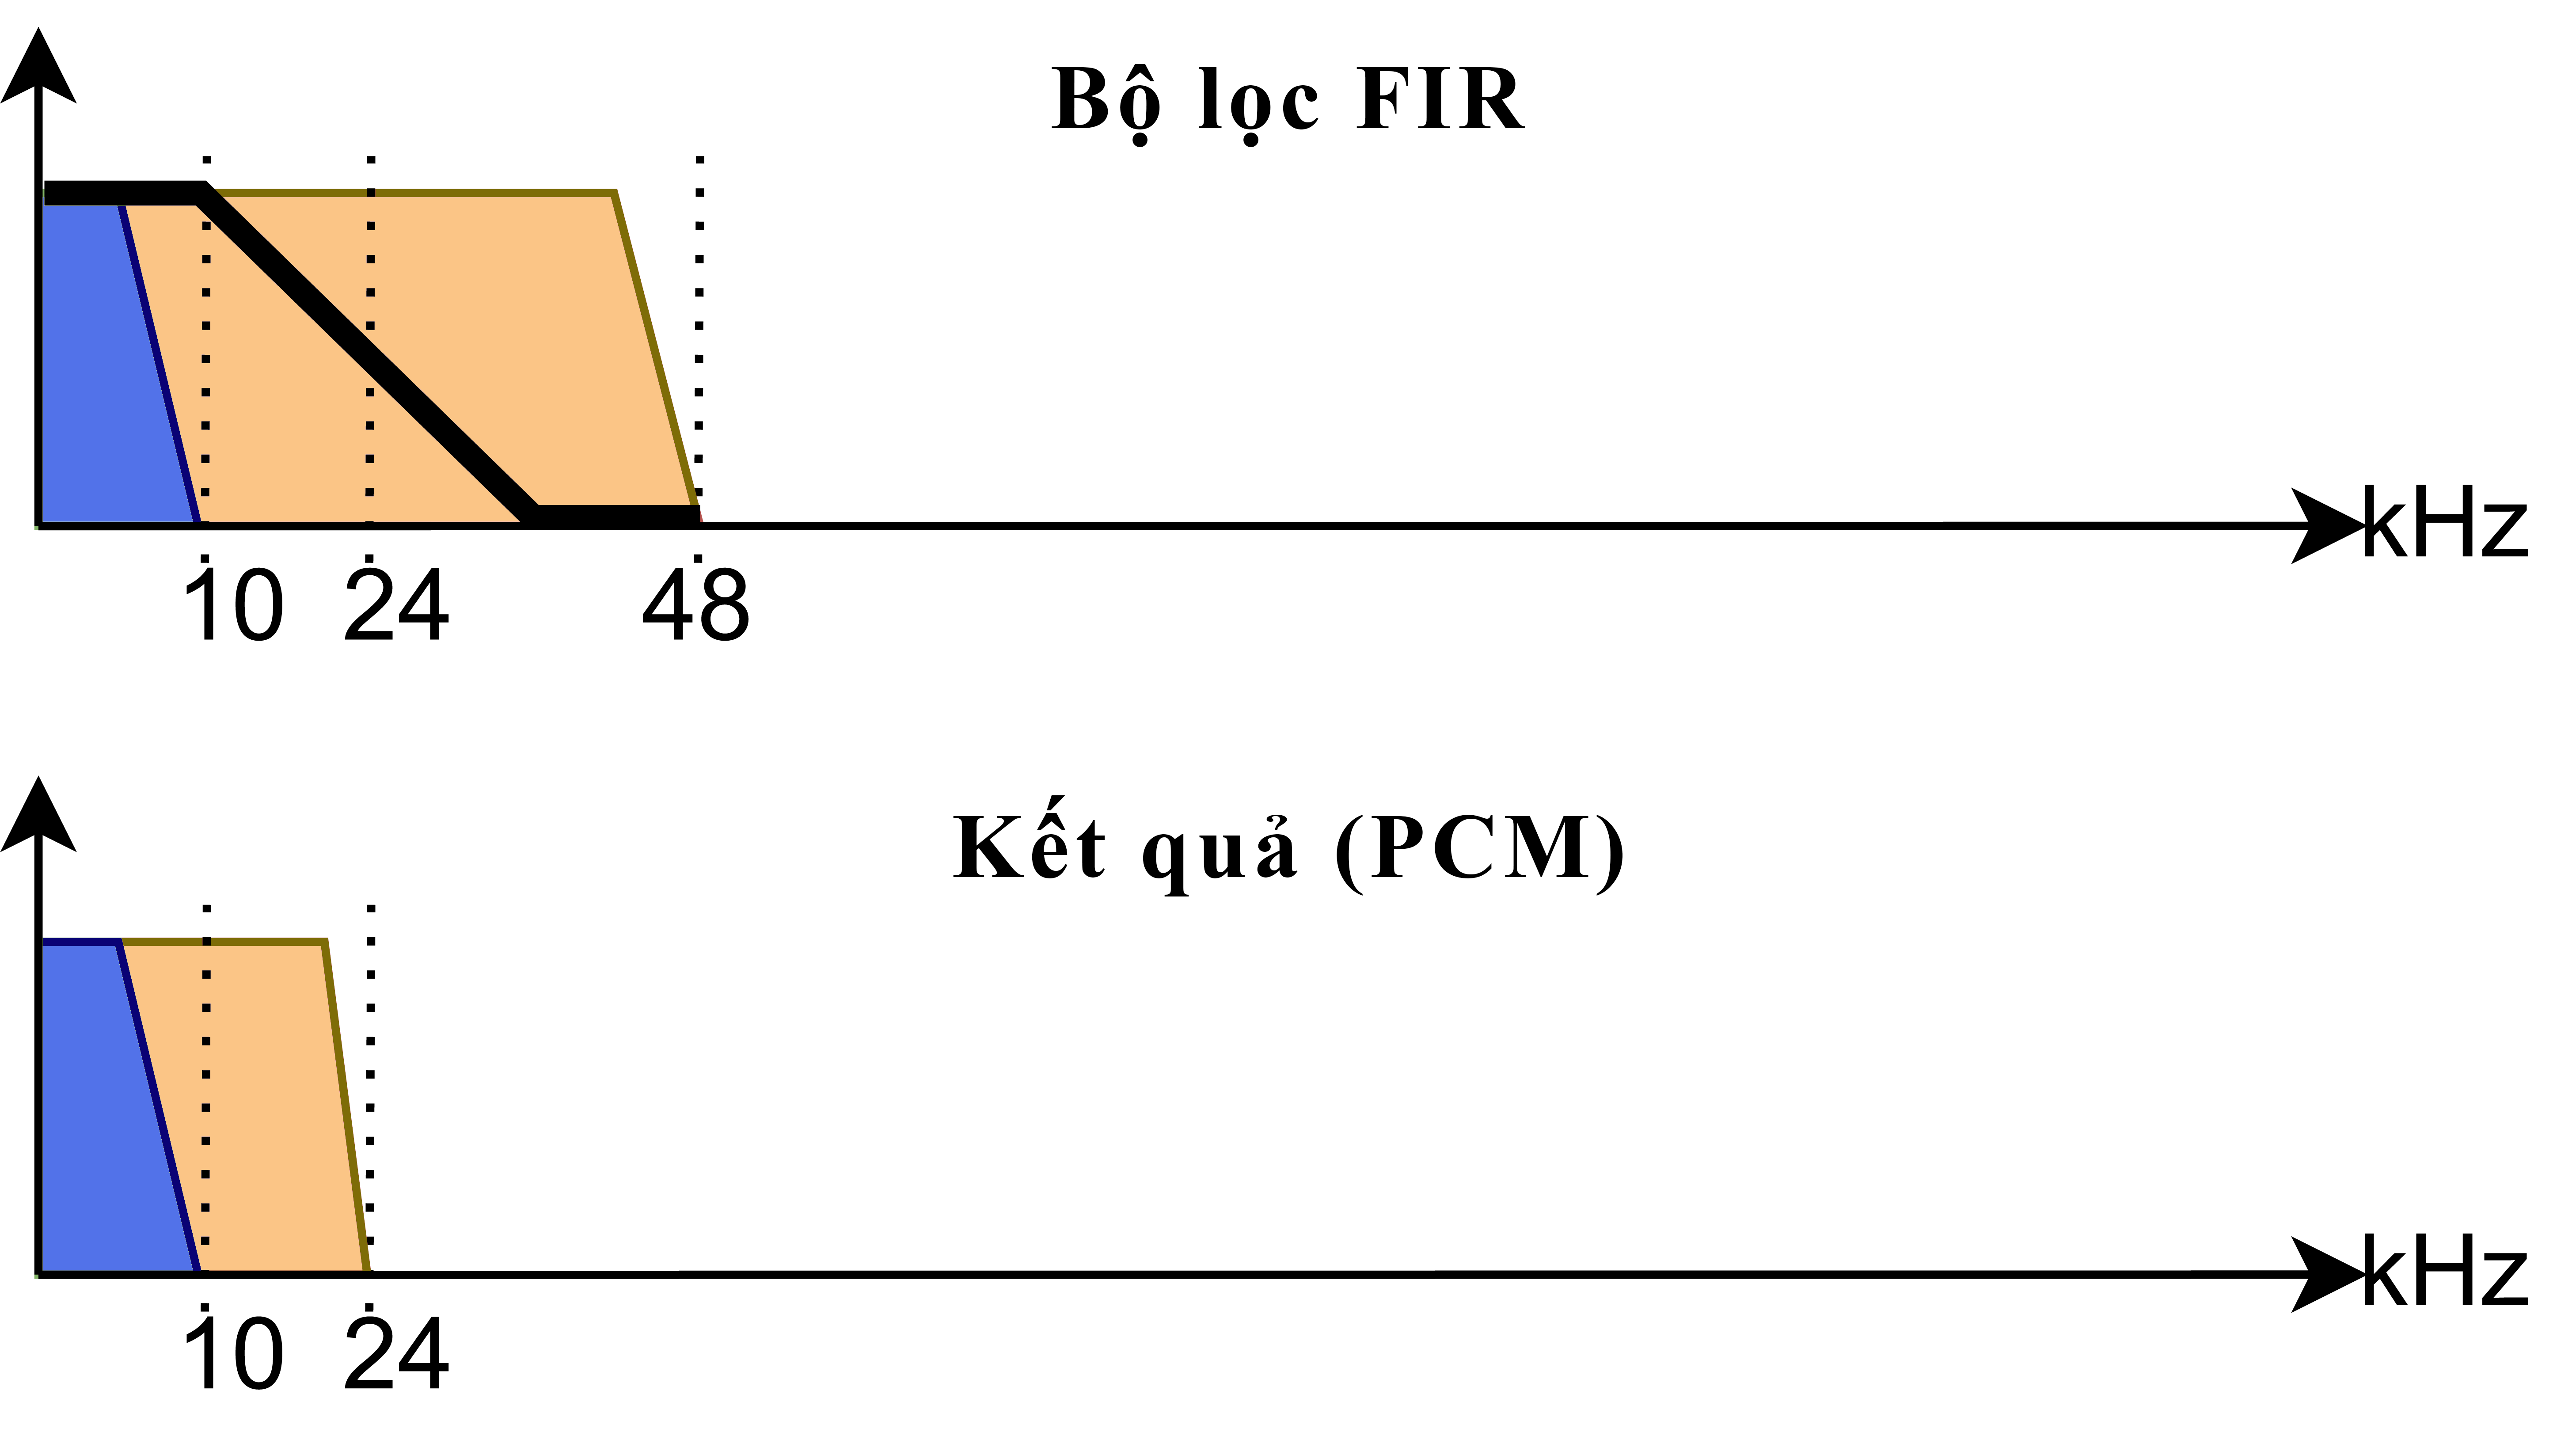
\includegraphics[width=11cm]{Images/Chuong3/4.png}
    \caption[Phổ của tín hiệu thu được cuối cùng]{\bfseries \fontsize{12pt}{0pt}\selectfont Phổ của tín hiệu thu được cuối cùng}
    \label{t4}
\end{figure}

Sau khi chạy thuật toán \textbf{Parks-McClellan/Remez} với các thông số đã nên ở trên, ta có đồ thị đáp ứng tần số, đáp ứng xung và số lượng taps của từng bộ lọc như hình \ref{a}, \ref{b}, \ref{c}, \ref{d}.  
\vspace{1.5cm}
\begin{figure}[H]
    \centering
    \includesvg[width=15.5cm]{Images/Chuong3/CIC.svg}
    \caption[Đáp ứng tần số và đáp ứng xung của bộ lọc CIC]{\bfseries \fontsize{12pt}{0pt}\selectfont Đáp ứng tần số và đáp ứng xung của bộ lọc CIC}
    \label{a}
\end{figure}
\vspace{1.5cm}
\begin{figure}[H]
    \centering
    \includesvg[width=15.5cm]{Images/Chuong3/HB1.svg}
    \caption[Đáp ứng tần số và đáp ứng xung của bộ lọc Half Band (1)]{\bfseries \fontsize{12pt}{0pt}\selectfont Đáp ứng tần số và đáp ứng xung của bộ lọc Half Band (1)}
    \label{b}
\end{figure}
\vspace{1.5cm}
\begin{figure}[H]
    \centering
    \includesvg[width=15.5cm]{Images/Chuong3/HB2.svg}
    \caption[Đáp ứng tần số và đáp ứng xung của bộ lọc Half Band (2)]{\bfseries \fontsize{12pt}{0pt}\selectfont Đáp ứng tần số và đáp ứng xung của bộ lọc Half Band (2)}
    \label{c}
\end{figure}
\begin{figure}[H]
    \centering
    \includesvg[width=15.5cm]{Images/Chuong3/FIR.svg}
    \caption[Đáp ứng tần số và đáp ứng xung của bộ lọc FIR]{\bfseries \fontsize{12pt}{0pt}\selectfont Đáp ứng tần số và đáp ứng xung của bộ lọc FIR}
    \label{d}
\end{figure}
\subsection{Mô phỏng và kiểm tra hệ thống}
Việc mô phỏng lại hệ thống sẽ triển khai bằng ngôn ngữ \textbf{Python}, sử dụng thư viện \textbf{Numpy} và \textbf{Scipy}.

Quá trình mô phỏng sẽ được thực hiện như sau: Tín hiệu đầu vào PDM sẽ được chập với đáp ứng xung của từng bộ lọc ở từng giai đoạn. Sau mỗi giai đoạn đó, số mẫu sẽ được giảm đi bằng với tỷ lệ Decimation đã được định sẵn (hình \ref{pipeline_new}).

Để tạo ra tín hiệu PDM, chúng ta phải tiến hành chuyển đổi tín hiệu ban đầu thông qua bộ điều chế Sigma-Delta bậc 4 và tỷ lệ Oversampling 48 bằng thư viện \textbf{deltasigma}.

\textbf{Kiểm tra}:

Cho đầu vào là tín hiệu 3 thành phần gồm 3 sóng sin có tần số lần lượt 4 kHz, 13 kHz, 22 kHz như phương trình \ref{3sin}.
\begin{equation} \label{3sin}
    x(t) = \frac{0.4}{3} (sin(2\pi \times 4000\times t) + sin(2\pi \times 13000\times t) + sin(2\pi \times 22000\times t))
\end{equation}

Tín hiệu này, sau đó sẽ đưa qua bộ điều chế Sigma-Delta. Chúng ta thu được tín hiệu ở miền thời gian và tần số như hình \ref{sd1} và \ref{sd2}.
\begin{figure}[H]
    \centering
    \includesvg[width=16.5cm]{Images/Chuong3/test/pdm_1.svg}
    \caption[Tín hiệu trên miền thời gian sau khi qua bộ điều chế]{\bfseries \fontsize{12pt}{0pt}\selectfont Tín hiệu trên miền thời gian sau khi qua bộ điều chế}
    \label{sd1}
\end{figure}

\begin{figure}[H]
    \centering
    \includesvg[width=16.5cm]{Images/Chuong3/test/psd_1.svg}
    \caption[Phổ mật độ công suất của tín hiệu PDM]{\bfseries \fontsize{12pt}{0pt}\selectfont Phổ mật độ công suất của tín hiệu PDM}
    \label{sd2}
\end{figure}

Hình \ref{sd1} mô tả tín hiệu đầu vào là đường màu đỏ và đường xanh là tín hiệu PDM sau khi được điều chế. Điều chúng cần quan tâm ở đây là phổ của tín hiệu PDM (\ref{sd2}). Chúng ta có thể dễ dàng quan sát được, 3 đường thẳng có độ lớn bất thường đó là tín hiệu chính tương ứng với 3 tần số được nêu trên. Nhiễu lượng tử được đẩy sang miền tần số cao (miền không cần quan tâm) và 1 phần cực kỳ nhỏ ở dải 0 - 24 kHz (có thể quan sát rõ ràng ở hình \ref{sd3}). Ở vùng cần thu tín hiệu, SNR lớn hơn 100 dB, điều này đã đáp ứng được với thông của micro MEMS.

\begin{figure}[H]
    \centering
    \includesvg[width=16.5cm]{Images/Chuong3/test/psd_2.svg}
    \caption[Phổ mật độ công suất của tín hiệu PDM (2)]{\bfseries \fontsize{12pt}{0pt}\selectfont Phổ mật độ công suất của tín hiệu PDM (2)}
    \label{sd3}
\end{figure}

Tiến hành mô phỏng, thu được tín hiệu ở bộ lọc FIR cuối cùng có biểu đồ ở miền thời gian như hình \ref{pcm_o}. Ở khoảng thời gian đầu, tín hiệu có vẻ bằng phẳng, đó là khoảng thời gian để nạp các tín hiệu cho các taps. Có vẻ các thành phần tần số 13 kHz và 23 kHz đã được loại bỏ. Để quan sát kỹ hơn, hãy quan sát biểu đồ mật độ công suất của tín hiệu PCM đầu ra.
\begin{figure}[H]
    \centering
    \includesvg[width=14cm]{Images/Chuong3/test/pcm_o.svg}
    \caption[Tín hiệu thu được sau mô phỏng]{\bfseries \fontsize{12pt}{0pt}\selectfont Tín hiệu thu được sau mô phỏng}
    \label{pcm_o}
\end{figure}

Hình \ref{psd_pcm} mô tả phổ của tín hiệu đầu ra của hệ thống. Có thể thấy bắt đầu từ điểm 6 kHz các thành tần số bắt đầu suy giảm mạnh. Chúng ta quan sát tần số có cường độ cao nhất trong miền 0 - 6 kHz, ban đầu (hình \ref{sd3}) là -17.5 dB và sau đó là -17.551 dB (hình \ref{psd_pcm}). Độ chênh lệch 0.051 đã đáp ứng đúng thông số độ gợn sóng của dải thông yêu cầu.

Đối với độ suy giảm của dải dừng, ở 2 vị trí 13 kHz và 23 kHz ban đầu có cường độ là -17.5 dB ngang với tín hiệu ở tần số 6 kHz cần thu. Sau khi đưa qua hệ thống, chúng giảm chỉ còn -114.404 dB, trong khi hệ thống chỉ yêu cầu độ suy hao là 89 dB. Các thành phần tần số không muốn được xem đã được loại bỏ. Phổ cũng bắt đầu suy giảm ổn định ở vị trí 10 kHz.
\begin{figure}[H]
    \centering
    \includesvg[width=16.5cm]{Images/Chuong3/test/psd_pcm.svg}
    \caption[Phổ của tín hiệu thu được (PCM)]{\bfseries \fontsize{12pt}{0pt}\selectfont Phổ của tín hiệu thu được (PCM)}
    \label{psd_pcm}
\end{figure}
\textbf{Kết luận}: Hệ thống đã hoạt động đúng với yêu cầu thiết kế đã đặt ra.

\subsection{Kết luận chương}

Qua \hyperref[chuong3]{chương 3}, chúng ta đã tiến hành chọn và thiết kế kiến trúc cho các bộ lọc trong hệ thống chuyển đổi nhiều giai đoạn. Việc mô phỏng và kiểm thử cũng cho ra kết quả đúng với yêu cầu đặt ra. Trong chương tiếp theo, chúng ta sẽ triển khai hệ thống trên bằng thiết kế số.
\newpage
